\documentclass{ctexart}

\usepackage{enumitem}
\usepackage{tcolorbox}
\usepackage{fancyvrb}%在 Verbatim 环境中使用 LaTeX 命令
\tcbuselibrary{skins}
\usepackage{colortbl}
\usepackage{geometry}
\geometry{margin = 1in}

\usepackage{fontspec}
\usepackage[colorlinks, linkcolor = red]{hyperref}
\def\mydollar{{\fontspec{Consolas}\$\ }}% 单个字体设置
\definecolor{structure}{RGB}{0,120,2}
\definecolor{main}{RGB}{0,166,82}
% \definecolor{main}{RGB}{0,120,2}
% \definecolor{main}{RGB}{59,180,5}
% \definecolor{main}{RGB}{150,150,150}
\definecolor{second}{RGB}{230,90,7}
\definecolor{white}{RGB}{255,255,255}

\newtcolorbox{mybox}[2][]{
    colframe = main,  
    colback = main!5,
    colbacktitle = main,
    coltitle = white, 
    title={#2},
    fonttitle=\bfseries,
    #1
}

\title{Git 学习笔记}
\author{ZiTai}
\date{\zhdate{2023/1/04}}

\begin{document}
\maketitle

\clearpage
\tableofcontents

\clearpage
\section{起步}
    作为编程小白,我们所接触到的代码都还很简单,一个人就可以完成对代码的开发、维护。
    但当我们涉及到多人合作开发时,就得思考一份代码如何保持同步?
    代码搞砸了如何回退到上一个版本?
    如此看来,所谓版本控制系统(Version Control System, VCS)
    就是一种记录一个或若干文件内容变化,以便将来查阅特定版本修改情况的系统。

\subsection*{本地版本控制系统}

\subsection*{集中化的版本控制系统(Centralized Version Control Systems, CVCS)}

\subsection*{分布式版本控制系统}
    常见的分布式版本控制系统(Distributed Version Control System, DVCS)有 Git、Mercurial、Bazaar 以及 Darcs 等,
    客户端不只是提取最新版本的文件快照,而且把代码仓库完整地镜像下来,包括完整的历史记录。
    如此一来,任何一处协同工作用的服务器发生故障,事后都可以用任何一个镜像出来的本地仓库恢复。
    因为每一次的克隆操作,实际上都是一次对代码仓库的的完整备份。

\clearpage
\section{Git 是什么?}
\subsection{直接记录快照,而非差异比较}
    Git 和其它版本控制系统(包括 Subversion 和近似工具)的主要差别在于 Git 对待数据的方式。
    从概念上来说,其它大部分系统以文件变更列表的方式存储信息,
    这类系统(CVS、Subversion、Perforce、Bazaar 等等)将它们存储的信息看作是一组基本文件和每个文件随时间积累的差异(它们通常称作\textbf{基于差异(delta-based)}的版本控制)。

    Git 却不是这样,它将数据看作是对小型文件系统的一系列快照。

\subsection{三种状态}
    Git 有三种状态,文件只会处于其中之一:

    \begin{enumerate}[labelindent=\parindent, leftmargin=*, align=left]
        \item 已修改(modified):表示修改了文件,但还没保存到数据库中。
        \item 已暂存(staged):表示对一个已修改文件的当前版本做了标记,使之包含在下次提交的快照中。
        \item 已提交(committed):表示数据已经安全地保存在本地数据库中。
    \end{enumerate}

    文件的这些状态会让 Git 项目拥有三个阶段:工作区、暂存区以及 Git 目录。

\begin{figure}[htbp]
    \centering
    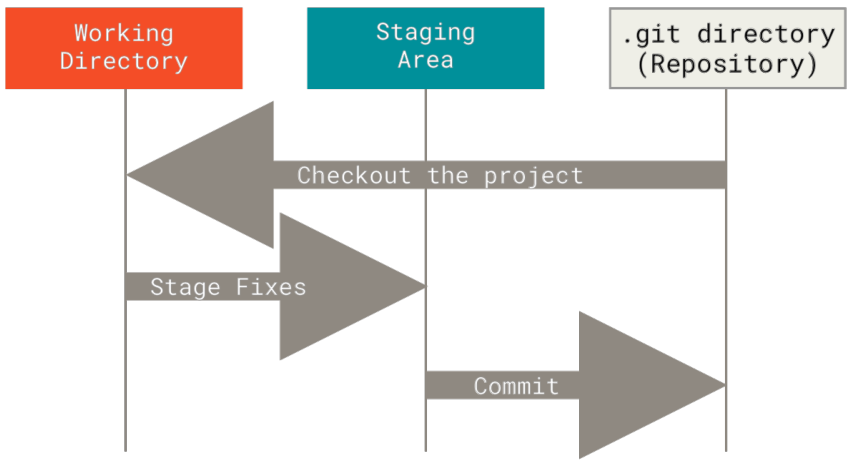
\includegraphics[width=0.80\textwidth]{pictures/01.png}
    \caption{工作区、暂存区以及 Git 目录(仓库)}
\end{figure}

    工作区是对项目的某个版本独立提取出来的内容。
    这些从 Git 仓库的压缩数据库中提取出来的文件,放在磁盘上供用户使用或修改。

    暂存区是一个文件,保存了下次将要提交的文件列表信息,一般在 Git 仓库目录中。
    按照 Git 的术语叫做“索引”,一般叫“暂存区”。

    Git 仓库目录是 Git 用来保存项目的元数据和对象数据库的地方。
    这是 Git 中最重要的部分,从其它计算机克隆仓库时,复制的就是这里的数据。

    基本的 Git 工作流程如下:

\begin{enumerate}[labelindent=\parindent, leftmargin=*, align=left]
    \item 在工作区中修改文件;
    \item 将你想要下次提交的更改选择性地暂存,这样只会将更改的部分添加到暂存区;
    \item 提交更新,找到暂存区的文件,将快照永久性存储到 Git 目录。
\end{enumerate}

\begin{figure}[htbp]
    \centering
    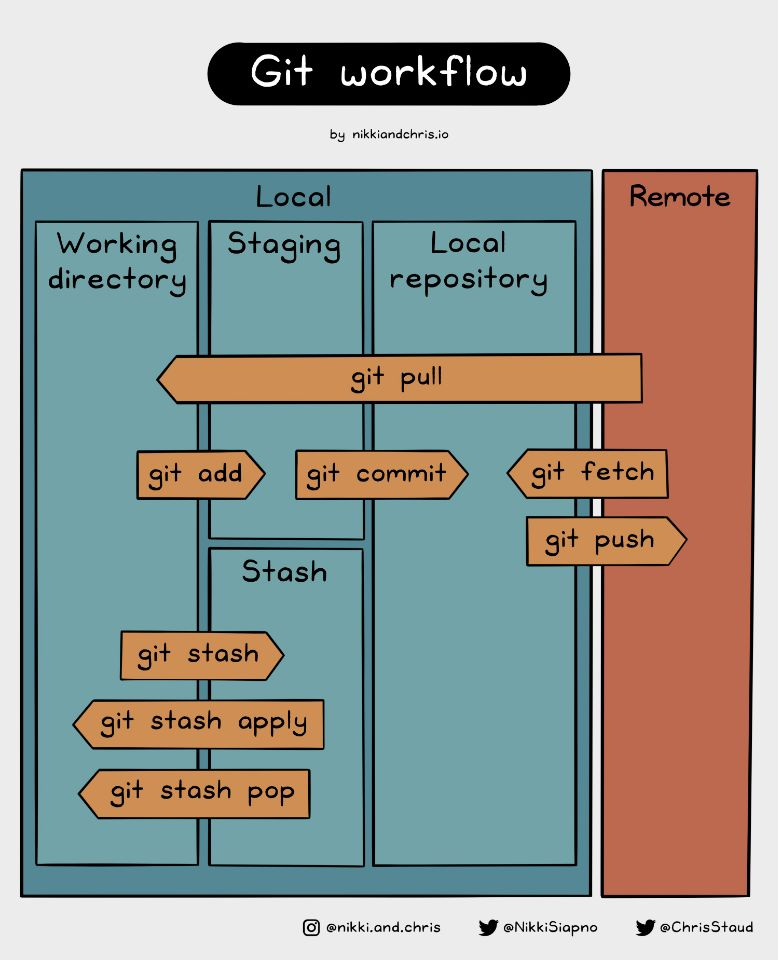
\includegraphics[width=0.45\textwidth]{pictures/03.jpg}
    \qquad
    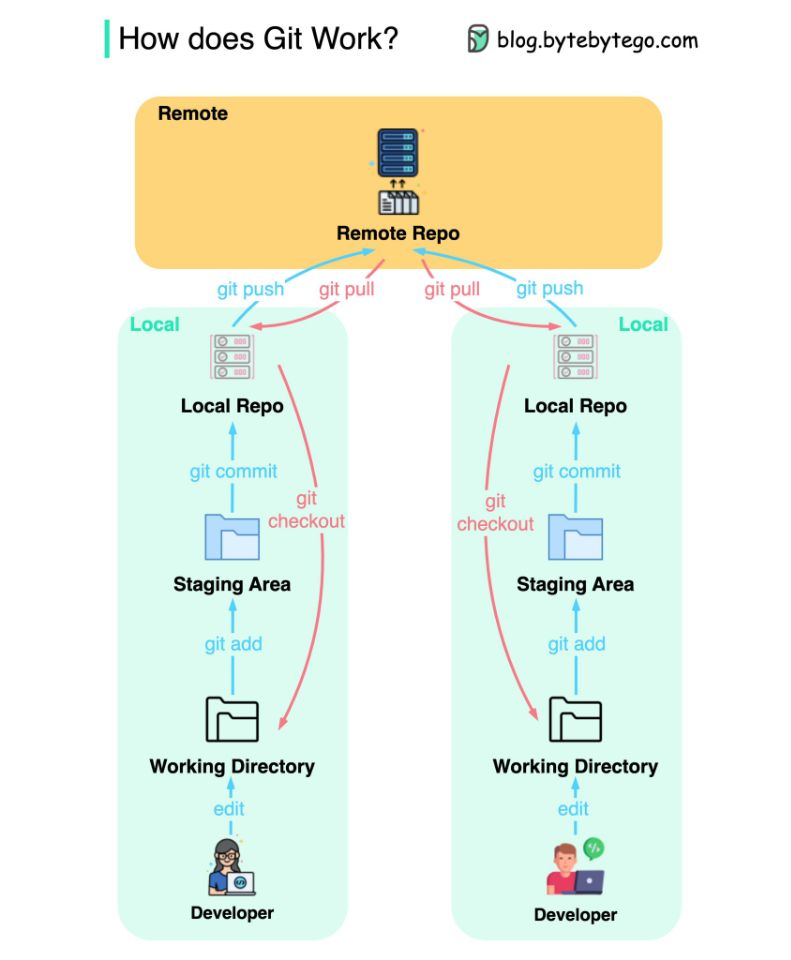
\includegraphics[width=0.45\textwidth]{pictures/05.jpg}
    \caption{Git 工作流}
\end{figure}

\begin{figure}[htbp]
    \centering
    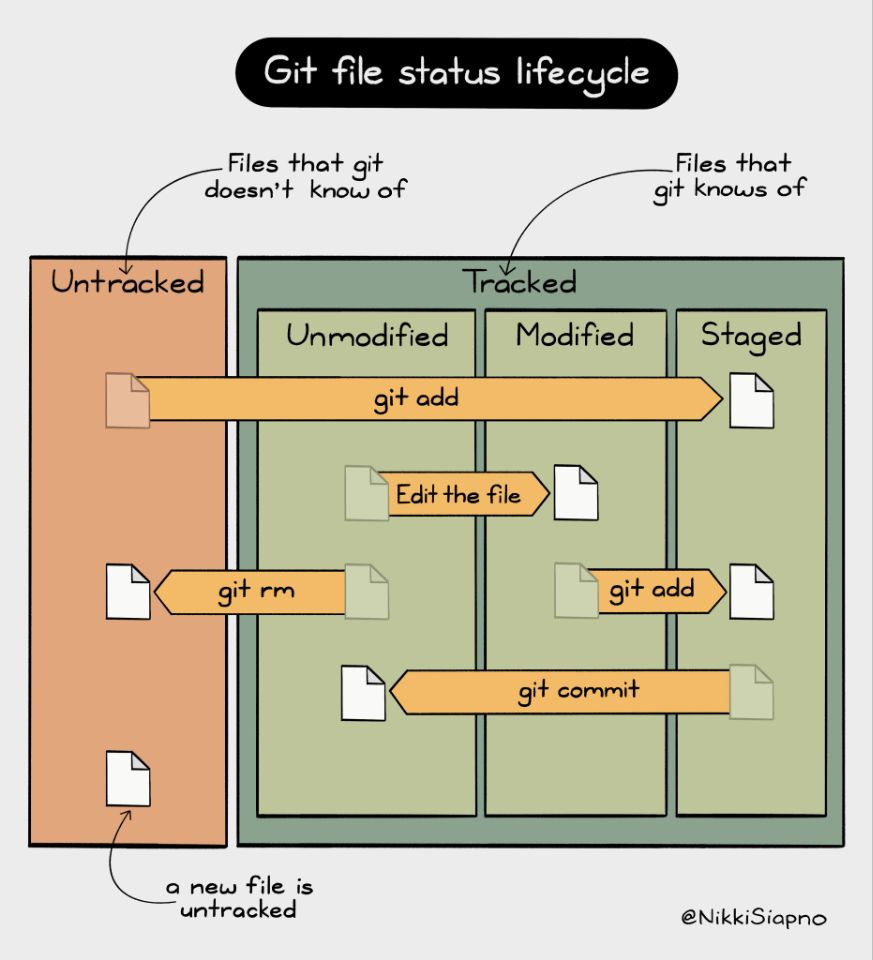
\includegraphics[width=0.80\textwidth]{pictures/04.jpg}
    \caption{Git 文件状态生命周期}
\end{figure}

\subsection{安装 Git}
\subsubsection{Arch Linux}
    \begin{mybox}{}
        \mydollar \texttt{sudo pacman -S git}
    \end{mybox}

\subsubsection{Windows}
    见 \href{https://git-scm.com/}{Git 官网}。

\subsection{初次运行 Git 前的配置}
    我们需要做几件事来定制 Git 环境。
    每台计算机上只需要配置一次,程序升级时会保留配置信息,可以在任何时候再次通过运行命令来修改它们。

    Git 自带一个 \verb|git config| 的工具来帮助设置控制 Git 外观和行为的配置变量。
    这些变量存储在三个不同的位置:

\begin{enumerate}[labelindent=\parindent, leftmargin=*, align=left]
    \item \verb|/etc/gitconfig| 文件:包含系统上每一个用户及它们仓库的通用配置。
          如果在执行 \verb|git config| 时带上 \verb|--system| 选项,那么它就会读写文件中的配置变量
          (由于它是系统配置文件,因此需要管理员或超级用户权限来修改它)。
    \item \verb|~/.gitconfig| 或 \verb|~/.config/git/config| 文件:只针对当前用户。可以传递 \verb|--global| 选项让 Git 读写此文件,这会对你系统上所有的仓库生效。
    \item 当前使用仓库的 Git 目录中的 \verb|config| 文件(即 \verb|.git/config| ):针对该仓库,可以传递 \verb|--local| 选项让 Git 强制读写此文件,虽然默认情况下用的就是它。(当然,你需要进入某个 Git 仓库中才能让该选项生效。)
\end{enumerate}

    每一个级别会覆盖上一级别的配置,所以 \verb|.git/config| 配置变量会覆盖 \verb|/etc/gitconfig| 中的配置变量。

    在 Windows 系统中,Git 会查找 {\fontspec{Consolas}\$}\verb|HOME| 目录下(一般情况是 \verb|C:\User\|{\fontspec{Consolas}\$}\verb|USER|)的 \verb|.gitconfig| 文件。

\subsection{用户信息}
    安装完 Git 后,需要做的第一件事就是设置用户名和邮件地址。
    每一个 Git 提交都会使用这些信息,它们会写入到每一次提交中,并不可更改:

\begin{mybox}{}
    \mydollar \texttt{git config --global user.name "Tom"}
    \tcbline
    \mydollar \texttt{git config --global user.email Tom@example.com}
\end{mybox}

    \textbf{注}:如果使用了 \texttt{--global} 选项,那么该命令只需要运行一次,以后 Git 都会使用这些信息。
    若想针对特定项目使用不同的用户名与邮件时,可以在该项目目录下运行不带 \texttt{--global} 选项的命令来配置。



\clearpage
\section{Git 常见工作流程}
\subsection{个人使用}
\subsubsection{本地管理}
    将个人电脑的磁盘作为本地仓库,而没有远程仓库。

    在想要创建项目的目录下,打开 git bash 命令行窗口,
    使用 \verb|git init| 命令即可初始化一个本地仓库。

\subsubsection{本地和远程管理}
    一般使用 Github 作为项目托管平台(远程仓库),
    先在 Github 上创建一个仓库(作为远程仓库),
    然后在电脑文件目录下打开 git bash 命令行窗口,
    使用 \verb|git clone <git_url>| 命令克隆仓库到本地。

\subsection{团队合作}
\subsubsection{受别人邀请参加项目}
% https://zhuanlan.zhihu.com/p/519343836
    以一个例子说明,受别人邀请参加一个项目时,该如何贡献代码。
    
    2023 年受邀参与 \href{https://github.com/latexstudio/LaTeXFAQ-cn}{LaTeXFAQ-cn} 项目。

    首先,\href{https://github.com/latexstudio}{仓库创建者} 在项目页面下打开“Settings”,
    点击“Collaborators”中的“Add people”,输入受邀人的 Github 用户名发起邀请,被邀人受到邮件后同意邀请。
    这时,被邀请人也有权限修改和提交仓库里的代码了。

    Collaborators 贡献代码的操作:

    \begin{mybox}{将远程仓库的一个分支克隆到本地}
        \mydollar \texttt{git clone -b <branch> <url>}
    \end{mybox}

    \begin{mybox}{进行 Collaborator 的用户名与邮箱的配置}
        \mydollar \texttt{git config user.name "Collaborators's name"}

        \mydollar \texttt{git config user.name "Collaborators's email"}
    \end{mybox}

    \begin{mybox}{更新远程仓库的修改}
        \mydollar \texttt{git pull}
    \end{mybox}

    \begin{mybox}{修改并提交自己的代码}
        \mydollar \texttt{git add somefile.cpp}

        \mydollar \texttt{git commit -m "Collaborators's push"}
        
        \mydollar \texttt{git push}
    \end{mybox}








\clearpage
\section{Git 常见命令}

\begin{mybox}{git bash 清屏操作}
    \mydollar \texttt{ctrl + L} 将滚动条至于最下方,滚动屏幕还是可以看到之前的命令
    \tcbline
    输入 \texttt{reset} 命令,再回车,真正清除屏幕上所有的内容
\end{mybox}

\begin{mybox}{获取帮助}
    使用 Git 需要获取帮助时,三个等价的方法找到 Git 命令的综合手册(manpage)

    \mydollar git help <verb>

    \mydollar git <verb> --help

    \mydollar man git-<verb>
    \tcbline
    \mydollar git help config

    获取 \verb|git config| 命令的手册
    \tcbline
    \mydollar git add -h

    如果不需要全面的手册,只需要可用选项的快速参考,
    可以使用 \verb|-h| 选项获得更简明的"help"。
    例如这条命令输出命令 \verb|add| 的快速参考
\end{mybox}

\clearpage
\subsection{配置 Git}

\begin{mybox}{检查 Git 配置}
    \mydollar \texttt{git config --list --show-origin}
    
    查看 Git 配置以及它们所在的文件
    \tcbline
    \mydollar \texttt{git config --list}
    
    检查 Git 配置,列出所有 Git 当时能找到的配置
    \tcbline
    \mydollar git config <key>
    
    检查 Git 的某一项配置,例如,检查用户名 \verb|git config user.name|
\end{mybox}

\begin{mybox}{配置 Git 默认文本编辑器}
    \mydollar \texttt{git config --global core.editor emacs}
    \tcbline

    Git 使用操作系统默认的文本编辑器,使用这条命令可以设置默认文本编辑器,例如使用 Emacs
\end{mybox}

\clearpage
\subsection{获取 Git 仓库}
    一般有两种方法获取 Git 仓库:
    
    \begin{enumerate}[labelindent=\parindent, leftmargin=*, align=left]
        \item 将尚未进行版本控制的本地目录转换为 Git 仓库(该目录既可以有文件,也可以没文件)。
        \item 从其它服务器克隆一个已存在的 Git 仓库。
    \end{enumerate}

    \begin{mybox}{在已存在目录中初始化仓库}
        \mydollar \texttt{git init}

        \mydollar \texttt{git init <project\_name>}
        \tcbline
        在当前目录下,该命令将创建一个名为 \texttt{.git} 的子目录。
        这个子目录含有初始化 Git 仓库中所有必须的文件。
        但这只是一个初始化操作,项目(目录)里的文件还没有被跟踪。
    \end{mybox}

    \begin{mybox}{克隆现有的仓库}
        \mydollar git clone <git\_url>
    
        \mydollar git clone <git\_url my\_directory>
        
        将项目克隆到指定的目录下
    \end{mybox}


% \subsection*{文件的状态变化周期}
% \begin{figure}[htbp]
%     \centering
%     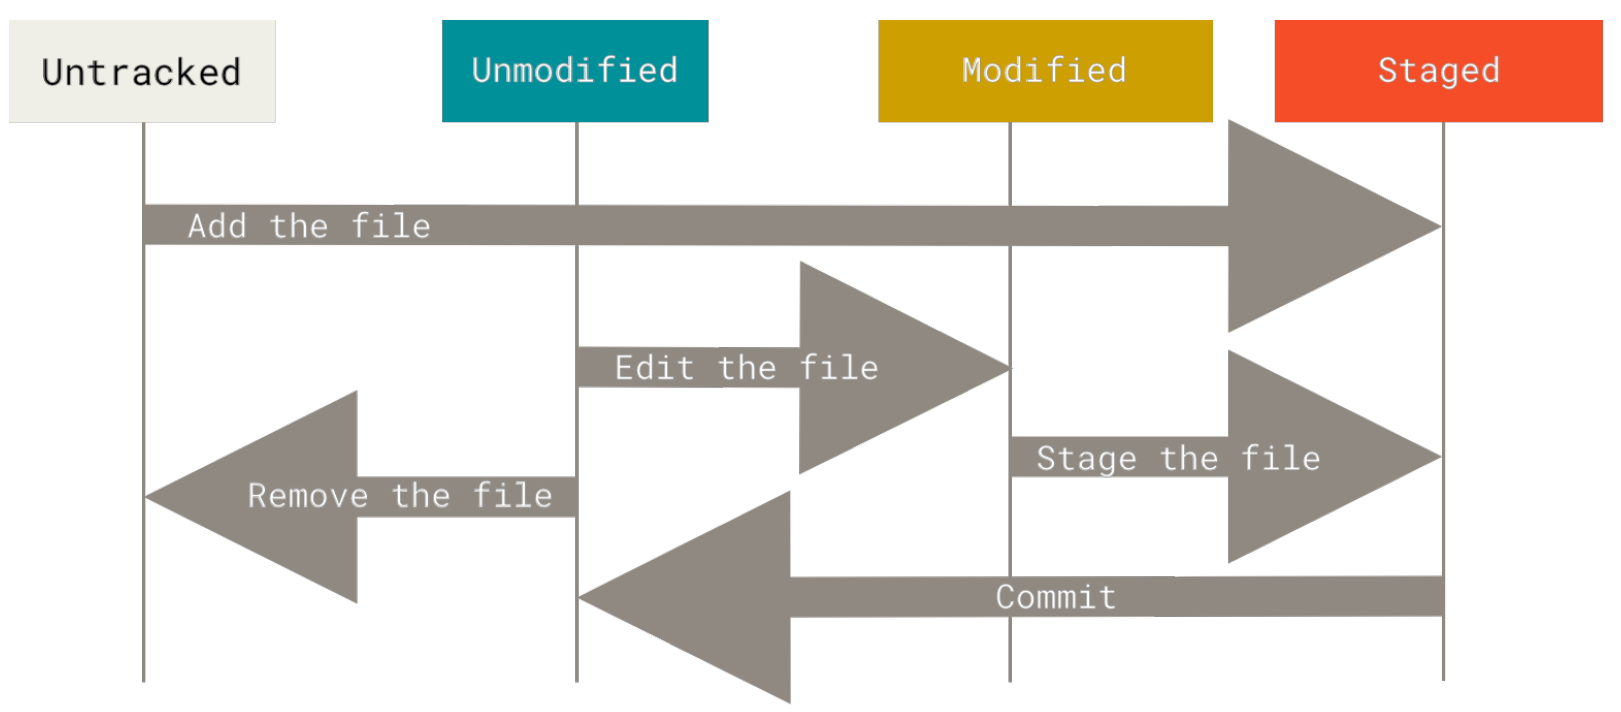
\includegraphics[width=0.80\textwidth]{pictures/02.png}
%     \caption{文件的状态变化周期}
% \end{figure}
\clearpage
\subsection{检查当前文件的状态}

\begin{mybox}{查看文件处于什么状态}
    \mydollar git status

    该命令的输出十分详细,有些繁琐。
    \tcbline
    \mydollar git status -s

    \mydollar git status --short

    格式更加紧凑的输出
    \tcbline
    \begin{enumerate}[labelindent=\parindent, leftmargin=*, align=left]
        \item 输出中有两栏,左栏指明了暂存区的状态,右栏指明了工作区的状态
        \item 新添加的未跟踪文件前面有??标记
        \item 新添加到暂存区中的文件前面有 A 标记
        \item 修改过的文件前面有 M 标记
        \item MM 表示文件暂存后又做了修改,因此改文件的修改中既有已暂存的部分,又有未暂存的部分
    \end{enumerate}
\end{mybox}


\begin{mybox}{查看已暂存和未暂存的修改}
    \mydollar git diff
\begin{enumerate}[labelindent=\parindent, leftmargin=*, align=left]
    \item 查看尚未暂存的文件更新了哪些部分,通过文件补丁的格式更加具体地显示哪些行发生了改变
    \item 此命令比较的是工作目录中当前文件和暂存区域快照之间的差异。也就是修改之后还没有暂存起来的变化内容
    \item \verb|git diff| 本身只显示尚未暂存的改动,而不是自上次提交以来所做的所有改动。所以有时候一下子暂存了所有更新过的文件,运行 \verb|git diff| 后却什么也没有,就是这个原因
\end{enumerate}

    \tcbline
    \mydollar git diff --staged

    \mydollar git diff --cached

    查看已暂存的将要添加到下次提交里的内容,此命令将比对已暂存文件与最后一次提交的文件差异(--staged 和 --cached 是同义词)。
\end{mybox}

\begin{mybox}{\mydollar git add <file\_name>}
    跟踪一个名为 file\_name 的文件
    \tcbline
    \verb|git add| 命令使用文件或目录的路径作为参数;如果参数是目录的路径,该命令将递归地跟踪该目录下的所有文件

    这是个多功能命令:可以用它开始跟踪新文件,或者把已跟踪的文件放到暂存区,还能用于合并时把有冲突的文件标记为已解决状态等。可以将这个命令理解为“精确地将内容添加到下一次提交中”而不是“将一个文件添加到项目中”
\end{mybox}


\begin{mybox}{\mydollar git ls-files}
    列出已跟踪的文件
    \tcbline
    \textbf{删除远程仓库的文件}

    \mydollar git rm --cached <file\_name>

    \mydollar git commit -m "something comment"

    \mydollar git push origin <branch\_name>
\end{mybox}


\begin{mybox}{提交更新}
    \mydollar git commit

    暂存区已经准备就绪时,就可以提交了,此时会启动已设置好的文本编辑器来输入提交说明。
    \tcbline
    \mydollar git commit -m “commit information”

    将提交信息与命令放在同一行
    \tcbline
    \mydollar git commit -a

    使用暂存区域的方式可以精心准备要提交的细节,但有时候这么做略显繁琐。此时可以使用 \verb|-a| 选项,来跳过使用暂存区域的方式:Git 会自动把所有已经跟踪过的文件暂存起来一并提交,从而跳过 \mydollar git add 步骤

    \verb|-a| \textbf{选项使本次提交包含了所有修改过的文件,有时这个选项会将不需要的文件添加到提交中}
\end{mybox}


\begin{mybox}{忽略文件}
    有时候,我们并不需要将目录下所有的文件都纳入 Git 管理,也希望它们总出现在未跟踪文件列表里。通常是一些自动生成的文件,例如日志文件,或者编译过程中创建的临时文件等。此时,可以创建一个名为 \verb|.gitignore| 的文件,在其中列出要忽略的文件的模式。
    \tcbline
    \verb|.gitignore| 文件的格式规范:
\begin{enumerate}[labelindent=\parindent, leftmargin=*, align=left]
    \item 所有空行或者以 \verb|#| 开头的行都会被 Git 忽略
    \item 可以使用标准的 glob 模式匹配,它会递归地应用在整个工作区中
    \item 匹配模式可以以(/)开头防止递归
    \item 匹配模式可以以(/)结尾指定目录
    \item 要忽略指定模式以外的文件或目录,可以在模式前加上(!)取反
\end{enumerate}
    其中,glob 模式是指 shell 所使用的的简化了的正则表达式

    星号(*)匹配零个或多个任意字符
    \tcbline
    一个 \verb|.gitignore| 文件的例子,
\begin{verbatim}
    *.[oa]
    *~
\end{verbatim}
    第一行告诉 Git 忽略所有以 \verb|.o| 或 \verb|.a| 结尾的文件\footnote{一般这类对象文件和存档文件都是编译过程中出现的。}。第二行告诉 Git 忽略所有名字以波浪符(\verb|~|)结尾的文件\footnote{许多文本编辑软件(比如 Emacs)都用这样的文件名保存副本。}。

    \textbf{更详细的} \verb|.gitignore| \textbf{文件列表}:\href{https://github.com/github/gitignore}{https://github.com/github/gitignore}
\end{mybox}


\begin{mybox}{移除文件}
    \mydollar git rm <file\_name>

    从 Git 中移除某个文件,也即从已跟踪文件清单中移除(从暂存区域移除),然后提交。此命令还会连带从工作目录中删除指定的文件,这样以后就不会出现在未跟踪文件清单中了
    \tcbline
    如果只是简单地从工作目录中手工删除文件(运行 \verb|rm <file\_name>|),然后再运行 \verb|git rm <file\_name>|,下一次提交时,该文件就不再纳入版本管理了
    \tcbline
    如果要删除之前修改过或已放到暂存区的文件,则必须使用强制删除选项 \verb|-f|,这是一种安全特性,用于防止误删尚未添加到快照的数据,这样的数据不能被 Git 恢复
    \tcbline
    \mydollar git rm --cached <file\_name>

    把文件从 Git 仓库中删除(从暂存区域移除),但仍然希望保留在当前工作目录中。换句话说,想让文件保留在磁盘,但并不想让 Git 继续跟踪。当忘记添加 \verb|.gitignore| 文件,不小心把一个很大的日志文件或一堆 \verb|.a| 这样的编译生成文件添加到暂存区时,可以使用这条命令。
    \tcbline
    \mydollar git rm \*~

    该命令会删除所有名字以~结尾的文件
\end{mybox}


\begin{mybox}{移动文件(更改文件名)}
    \mydollar git mv file\_from file\_to

    更改文件名
    \tcbline
    等价于运行三条命令:

    \mydollar mv file\_from file\_to

    \mydollar git rm file\_from

    \mydollar git add file\_to
\end{mybox}


\begin{mybox}{查看提交历史}
    \mydollar git log

    不传入任何参数的默认情况下,该命令按时间先后顺序列出所有的提交,最近的更新排在最上面。这条命令会列出每个提交的 SHA-1 校验和、作者的名字和电子邮件、提交时间以及提交说明
    \tcbline
    \mydollar git log -p 或 git log --patch

    显示每次提交所引入的差异(按补丁的格式输出)。

    也可以再加入“-2”选项来限制显示的日志条目数量,只显示最近的两次提交
    \tcbline
\end{mybox}

\begin{tabular}{| l | l |}
    \hline
    选项                &说明\\
    \hline
    -p                  &按补丁格式显示每个提交引入的差异\\
    \hline
    --stat              &显示每次提交的文件修改统计信息\\
    \hline
    --shortstat         &只显示 --stat 中最后的行数修改添加移除统计\\
    \hline
    --name-only         &仅在提交信息后显示已修改的文件清单\\
    \hline
    --name-status       &显示新增、修改、删除的文件清单\\
    \hline
    --abbrev--commit    &仅显示 SHA-1 校验和所有 40 个字符中的前几个字符\\
    \hline
    --relative-date     &使用较短的相对时间而不是完整格式显示日期\\
    \hline
    --graph             &在日志旁以 ASCII 图形显示分支与合并历史\\
    \hline
    --pretty            &使用其他格式显示历史提交信息。可用的选项包括 oneline、short、\\ & full、fuller和 format(用来定义自己的格式)\\
    \hline
    --oneline           &--pretty=oneline --abbrev-commit 合用的简写\\
    \hline
\end{tabular}


\begin{mybox}{远程仓库}
    远程仓库是指托管在因特网或其他网络中的你的项目的版本库。与他人协作涉及管理远程仓库以及根据需要推送或拉取数据

    \textbf{远程仓库可以在你的本地主机上}
\end{mybox}

\begin{mybox}{\mydollar git remote}
    查看你已经配置的远程仓库服务器。该命令会列出指定的每一个远程服务器的简写

    如果已经克隆了自己的仓库,那么至少应该看到 origin:这是 Git 克隆的仓库服务器的默认名字
    \tcbline
    \mydollar git remote -v

    显示需要读写远程仓库使用的 Git 保存的简写与其对应的 URL(可以使用不同的协议)
\end{mybox}


\begin{mybox}{\mydollar git remote add <short\_name> <url>}
    添加一个新的远程 Git 仓库,同时指定一个方便使用的简写(此时会用 <short\_name> 替代默认的远程仓库名 origin)
\end{mybox}


\begin{mybox}{\mydollar git fetch <remote>}
    从远程仓库获取数据:访问远程仓库,从中拉取所有你还没有的数据。执行完成后,你将拥有那个远程仓库中所有分支的引用,可以随时合并或查看
    \tcbline
    如果使用 \verb|clone| 命令克隆一个仓库,命令会自动将其添加为远程仓库并默认以“origin”为简写。所有,\verb|git fetch origin| 会抓取克隆(或上一次抓取)后新推送的所有工作。
    \tcbline
    \verb|git fetch| 命令只会将数据下载到本地仓库,并不会自动合并或修改你当前的工作,当准备好时必须手动将其合并入自己的工作
\end{mybox}


\begin{mybox}{\mydollar git pull}
    如果当前分支设置了跟踪远程分支,则该命令会自动抓取数据后合并该远程分支到当前分支。
    \tcbline
    默认情况下,\verb|git clone| 命令会自动设置本地 master 分支跟踪克隆的远程仓库的 master 分支(或其它名字的默认分支)。运行 \verb|git pull| 通常会从最初克隆的服务器上抓取数据并自动尝试合并到当前分支
\end{mybox}


\begin{mybox}{\mydollar git push <remote> <branch>}
    当你想分享你的项目时,必须将其推送到上游\footnote{上游:使用河流类比来说明数据流,上游是指将你的数据发送回河流的来源。当你向上游发送内容时,你将其发送回存储库的原始作者。}。当你想将 master 分支推送到 origin 服务器时(这两个名字是在克隆时自动设置好的名字),那么运行这个命令就可以将你所做的备份到服务器:\verb|git push origin master|

    \textbf{只有当你有克隆服务器的写入权限,并且之前没有人推送过时,这条命令才能生效}
\end{mybox}


\begin{mybox}{\mydollar git remote show <remote>}
    查看某一个远程仓库的更多信息
\end{mybox}


\begin{mybox}{远程仓库的重命名与移除}
    例如,想要将 pb 重命名为 paul,可以这样做:
\begin{Verbatim}[commandchars=\\\{\}]
    \mydollar \!\!git remote rename pb paul
    \mydollar \!\!git remote
    origin
    paul
\end{Verbatim}
    这条命令同样会修改你所有远程跟踪的分支名字。那些过去引用 \verb|pb/master| 的现在会引用 \verb|paul/master|
    \tcbline
    \mydollar git remote remove <name> 或 \mydollar git remote rm <name>

    移除一个远程仓库(比如,你已经从服务器上搬走了或不再想使用某一个特定的镜像了,又或者某一个贡献者不再贡献了)。使用这条命令删除一个远程仓库,那么所有和这个远程仓库相关的远程跟踪分支以及配置信息也会一起被删除
\end{mybox}



\begin{mybox}{标签}
    Git 支持两种标签:
\begin{enumerate}[labelindent=\parindent, leftmargin=*, align=left]
    \item 轻量标签(lightweight):很像一个不会改变的分支--它只是某个特定提交的引用。本质上是将提交校验和存储到一个文件中--没有保存任何其他信息
    \item 附注标签(annotated):存储在 Git 数据库中的一个完整对象,它们是可以被校验的,其中包含打标签者的名字、电子邮件地址、日期时间,此外还有一个标签信息,并且可以使用 GNU Privacy Guard(GPG)签名并验证。如果只是想用一个临时的标签,或者因为某些原因不想要保存这些信息,可以使用轻量标签
\end{enumerate}
    Git 可以给仓库历史中某一个提交打上标签,以示重要。人们会使用这个功能来标记发布结点(v1.0、v2.0 等)
\end{mybox}


\begin{mybox}{打标签}
    \textbf{查看标签}

    \mydollar git tag

    列出已有的标签
    \tcbline
    \mydollar git tag -l “v1.8.5*” 或 \mydollar git tag --list “v1.8.5*”

    列出所有 v1.8.5 系列的标签(* 是通配符)
    \tcbline
    \mydollar git show <tag\_name>

    查看标签信息和与之对应的提交信息:显示输出打标签者的信息、打标签的日期时间、附注信息,然后显示具体的提交信息
    \tcbline
    \textbf{创建附注标签}

    \mydollar git tag -a v1.4 -m "my version 1.4"

    创建一个附注标签,其中,\verb|-b| 选项指定了一条将会存储在标签中的信息。如果没有为附注标签指定一条信息,Git 会启动编辑器要求你输入信息
    \tcbline
    \textbf{创建轻量标签}

    \mydollar git tag <tag\_name>

    创建一个名为\ "<tag\_name>" 的轻量标签
    \tcbline
    \textbf{后期打标签}
    \tcbline
    \textbf{共享标签}
    \tcbline
    \textbf{删除标签}

    \mydollar git tag -d <tag\_name>

    删除本地上的一个轻量标签。此命令不会从任何远程仓库中移除这个标签

    但可以使用 \verb|git push <remote> :refs/tags/<tag\_name>| 来更新远程仓库,从而删除标签
    \tcbline
    \mydollar git push origin --delete <tag\_name>

    删除远程标签
    \tcbline
    \textbf{检出标签}
    
    \mydollar git checkout <tag\_name>

    查看某个标签所指向的文件版本。但这样会使仓库处于“分离头指针(detached HEAD)”的状态,这个状态有些不好的副作用
\end{mybox}


\begin{mybox}{Git 别名}
    通过 \verb|git config| 文件为每一个命令设置一个别名,这样就不用每次都输入完整的 Git 命令。例如,
\begin{Verbatim}[commandchars=\\\{\}]
    \mydollar \!\!git config --global alias.co checkout
    \mydollar \!\!git config --global alias.br branch
    \mydollar \!\!git config --global alias.ci commit
    \mydollar \!\!git config --global alias.st status
\end{Verbatim}
    这意味着,当要输入 \verb|git commit| 时,只需输入 \verb|git ci|。还可以利用这条命令“创建”属于自己的 Git 命令
\end{mybox}


\begin{mybox}{分支}
    Git 的分支,本质上是指向提交对象的可变指针。Git 默认分支名字是 master。多次提交后,就会产生一个指向最后那个提交对象的 master 分支。master 分支会在每次提交时自动向前移动
    \tcbline
    Git 的 master 分支并不是一个特殊的分支。它和其它分支完全没有区别。它只是 \verb|git init| 命令默认创建它时,大多数人懒得去改动它
\end{mybox}


\begin{mybox}{git 分支}
    \textbf{创建分支}

    \mydollar git branch <branch\_name>

    创建一个新分支:它创建了一个可移动的新的指针。该命令只会创建一个新分支,并不会自动切换到新分支中去,即你仍然在原分支上(HEAD 指针指向此时所在的分支)
    \tcbline
    \mydollar git branch -v
    
    查看每一个分支的最后一次提交
    \tcbline
    \mydollar git branch --merged
    
    查看哪些分支已经合并到当前分支
    \tcbline
    \mydollar git branch --no-merged
    
    查看所有包含未合并工作的分支
    \tcbline
    选项 \verb|--merged| 和 \verb|--no-merged| 在没有给定提交或分支名作为参数时,分别列出已合并或未合并到\textbf{当前}分支的分支

    可以附加一个参数来查看其它分支的合并状态而不必检出它们,例如,在 testing 分支中,查看 master 分支的合并情况:
\begin{Verbatim}[commandchars=\\\{\}]
    \mydollar \!\!git checkout testing
    \mydollar \!\!git branch --no-merged master
\end{Verbatim}
    \tcbline
    \textbf{切换分支}

    \mydollar git checkout <branch\_name>

    切换到\ "<branch\_name>" 分支上(此时 HEAD 指向了 <branch\_name>)

    注:分支切换会改变工作目录中的文件
    \tcbline
    \mydollar git log --oneline --decorate --graph --all

    输出提交历史、各个分支的指向以及项目的分支分叉情况
    \tcbline
    \mydollar git checkout -b <new\_branch\_name>

    创建新分支并立即切换过去
    \tcbline
    \textbf{合并分支}

    \mydollar git merge <branch\_name>

    将 <branch\_name> 分支合并到现在所处的分支上
    \tcbline
    \textbf{删除本地分支}

    \mydollar git branch -d <branch\_name>

    删除名为 <branch\_name> 的分支
    \tcbline
    \textbf{删除远程分支}

    \mydollar git push origin --delete <branch\_name>
\end{mybox}


\end{document}
